\documentclass[a4paper,12pt]{report}

\usepackage{cmap}
\usepackage[T2A]{fontenc}
\usepackage[utf8]{inputenc}
\usepackage[english,russian]{babel}
\usepackage{listings}
\usepackage{amsmath}
\usepackage{amsfonts}
\usepackage{float}
\usepackage{csquotes}
\usepackage{hyphenat}

% \usepackage{titlesec}
% \newcommand{\sectionbreak}{\clearpage}

\usepackage{graphicx}
\graphicspath{ {./images/} }

\usepackage{xcolor}
% \usepackage{courier}

\definecolor{buzzlightyear}{HTML}{8757A5}
\definecolor{grass}{HTML}{738D06}
\definecolor{sand}{HTML}{F18A2B}
\definecolor{comment}{HTML}{8E908B}

\lstdefinestyle{habrstyle}{
    backgroundcolor=\color{white},   
    commentstyle=\color{comment},
    keywordstyle=\bfseries\color{buzzlightyear},
    numberstyle=\tiny\color{comment},
    stringstyle=\color{grass},
    basicstyle=\ttfamily\footnotesize,
    breakatwhitespace=false,         
    breaklines=true,                 
    captionpos=b,                    
    keepspaces=true,                 
    numbers=left,                    
    numbersep=5pt,                  
    showspaces=false,                
    showstringspaces=false,
    showtabs=false,                  
    tabsize=4
}

\lstset{style=habrstyle}

\author{Луняк Николай}
\title{Лабораторная работа 2}
\date{\today}

\begin{document}
    \maketitle
    \tableofcontents
    \listoffigures
    \lstlistoflistings
    
    \chapter{Пробуем примеры из \texttt{chap02.ipynb}}
    
    Тут надо просто посмотреть на примеры из второй главы, послушать всякие звуки и убедиться, что все работает.
    
    \begin{figure}[H]
        \centering
        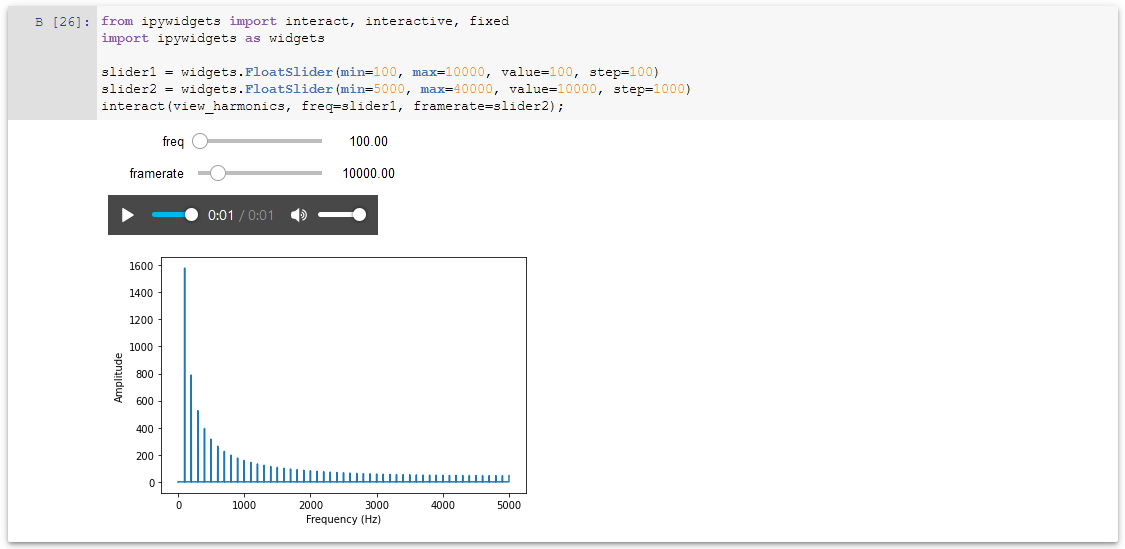
\includegraphics[width=\textwidth]{ex1_it_works.png}
        \caption{Работает}
        \label{fig:ex1_it_works}
    \end{figure}
    
    \chapter{Делаем \texttt{SawtoothSignal}}
    
    \section{Основной код}
    
    В задании просят за основу взять \texttt{Signal}, но в самой главе приводят примеры создания треугольного и прямоугольного сигналов на основе \texttt{Sinusoid}. Скорее всего, в задании опечатка, поэтому я буду пользоваться так же \texttt{Sinusoid} (иначе придется реализовывать и конструктор, чтобы передавать ему частоту).
    
\begin{lstlisting}[language=Python,caption=Реализация своего пилообразного сигнала]
from thinkdsp import Signal, Sinusoid, normalize, unbias, PI2

import numpy as np

class MySawtooth(Sinusoid):
    def evaluate(self, ts):
        cycles = self.freq * ts + self.offset / PI2
        frac, _ = np.modf(cycles)
        ys = self.amp * frac 
        return ys
\end{lstlisting}

    Надо еще убедиться, что он работает корректно.
    
\begin{lstlisting}[language=Python,caption=Проверка]
from thinkdsp import decorate

test_saw = MySawtooth(200)
test_wave = test_saw.make_wave(
    test_saw.period*3, 
    framerate=10000
)
test_wave.plot()
decorate(xlabel='Time (s)')
\end{lstlisting}

    \begin{figure}[H]
        \centering
        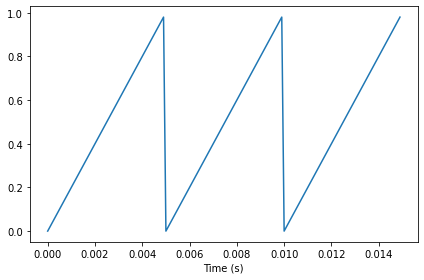
\includegraphics[width=\textwidth]{ex2_sawtooth_test.png}
        \caption{Результат}
        \label{fig:ex2_sawtooth_test}
    \end{figure}
    
    \section{Строим спектр}
    
\begin{lstlisting}[language=Python,caption=Построение спектра]
test_spectrum = test_wave.make_spectrum()
test_spectrum.plot()
decorate(xlabel='Frequency (Hz)')
\end{lstlisting}

    \begin{figure}[H]
        \centering
        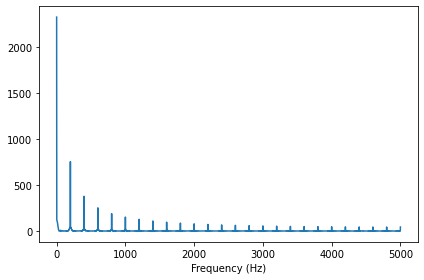
\includegraphics[width=\textwidth]{ex2_spectrum.png}
        \caption{Спектр}
        \label{fig:ex2_spectrum}
    \end{figure}
    
    В данном сигнале у нас как присутствуют \textquote{четнократные} частоты, так и их амлитуды уменьшаются пропорционально самой частоте, а не ее квадрату.
    
    \chapter{Проверка квадратного сигнала}
    
\begin{lstlisting}[language=Python,caption=Строим квадратный сигнал]
from thinkdsp import SquareSignal

signal = SquareSignal(1100)
wave = signal.make_wave(duration=0.5, framerate=10_000)
spectrum = wave.make_spectrum()
spectrum.plot()
\end{lstlisting}

    \begin{figure}[H]
        \centering
        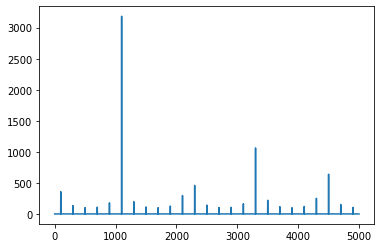
\includegraphics[width=\textwidth]{ex3_square_spectrum.png}
        \caption{Спектр}
        \label{fig:ex3_square_spectrum}
    \end{figure}
    
    Чтобы понять, слышно ли эти \textquote{\texttt{aliased}-частоты}, можно создать новый сигнал с более хорошей частотой дискретизации и сравнить.
    
\begin{lstlisting}[language=Python,caption=Строим квадратный сигнал]
wave2 = signal.make_wave(
    duration=0.5, 
    framerate=signal.freq*10
)
spectrum2 = wave2.make_spectrum()
spectrum2.plot()
\end{lstlisting}

    \begin{figure}[H]
        \centering
        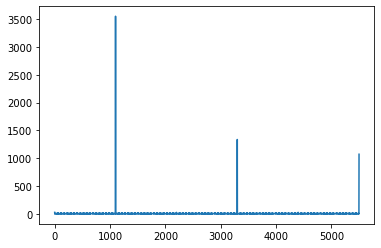
\includegraphics[width=\textwidth]{ex3_better_signal.png}
        \caption{Спектр почище}
        \label{fig:ex3_better_signal}
    \end{figure}
    
    На слух разница заметна, а значит мы действительно можем расслышать эти частоты.
    
    \chapter{Нулевая частота}
    
    \section{Создаем сигнал}
    
\begin{lstlisting}[language=Python,caption=Создаем сигнал]
from thinkdsp import TriangleSignal

signal = TriangleSignal(440)
wave = signal.make_wave(duration=0.01, framerate=11025)
wave.plot()
\end{lstlisting}

    \begin{figure}[H]
        \centering
        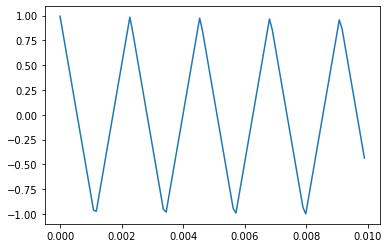
\includegraphics[width=\textwidth]{ex4_first.png}
        \caption{Первый сигнал}
        \label{fig:ex4_first}
    \end{figure}
    
    \section{Смотрим на \texttt{spectrum.hs[0]}}
    
    Видим: \texttt{1.0436096431476471e-14+0j}. \textquote{Длинна} этого комплексного числа описывает амплитуду нулевой компоненты разложения, а угол с $Re$ - сдвиг по фазе, то есть, частоту.
    
    \section{Зануляем}
    
\begin{lstlisting}[language=Python,caption=\textquote{Зануленный} сигнал]
spectrum.hs[0] = 0
wave2 = spectrum.make_wave()
wave2.plot()
\end{lstlisting}

    \begin{figure}[H]
        \centering
        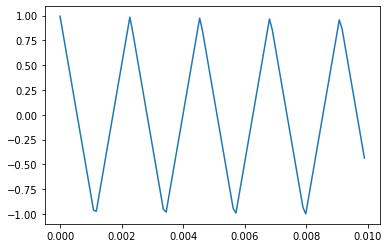
\includegraphics[width=\textwidth]{ex4_second.png}
        \caption{Новый сигнал}
        \label{fig:ex4_second}
    \end{figure}
    
    Как можно видеть, никакой разницы нет.
    
    \chapter{Делим амплитуду на частоту}
    
    Сама функция имеет следующий вид.
    
\begin{lstlisting}[language=Python,caption=Функция трансформации компонент]
def modify(spectrum):
    for it in range(1, len(spectrum.hs)):
        spectrum.hs[it] /= spectrum.fs[it]
    spectrum.hs[0] = 0
\end{lstlisting}

    Для ее проверки я создам пилообразный сигнал.
    
\begin{lstlisting}[language=Python,caption=Исходный сигнал]
from thinkdsp import SawtoothSignal

signal = SawtoothSignal(440)
wave = signal.make_wave(duration=0.5, framerate=440 * 100)
spectrum = wave.make_spectrum()
spectrum.plot()
\end{lstlisting}

    \begin{figure}[H]
        \centering
        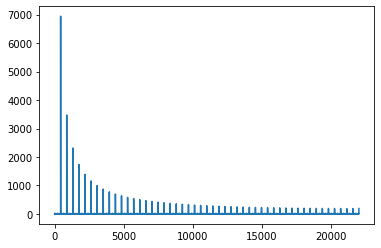
\includegraphics[width=\textwidth]{ex5_source.png}
        \caption{Исходный сигнал}
        \label{fig:ex5_source}
    \end{figure}
    
    Можно заметить, что амплитуды соответствующих компонент итак уменьшаются достаточно быстро, а, учитывая что внутри \texttt{modify()} будет производиться деление на $440k$ ($k \in \mathbb{Z}$), очень многие компоненты окажутся сильно подавленными.
    
\begin{lstlisting}[language=Python,caption=После \texttt{modify()}]
modify(spectrum)
spectrum.plot(high=100)
\end{lstlisting}

    \begin{figure}[H]
        \centering
        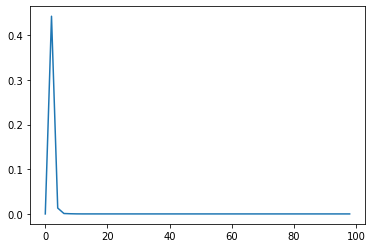
\includegraphics[width=\textwidth]{ex5_modified.png}
        \caption{Измененный сигнал}
        \label{fig:ex5_modified}
    \end{figure}
    
    Если прослушать этот сигнал через \texttt{spectrum.make\_wave().make\_audio()}, мы, действительно, ничего не услышим. Возможно, стоило попробовать с \texttt{SawtoothSignal}, ведь умплитуды компонент у него спадают обратно частоте а не ее квадрату.
    
    \chapter{Ищем загадочный сигнал}

    Возьмем пилообразный сигнал, применив написанную ранее \texttt{modify()}.
    
\begin{lstlisting}[language=Python,caption=Новый сигнал]
signal = SawtoothSignal(100)
wave = signal.make_wave(
    duration=signal.period*10, 
    framerate=10_000
)
wave.plot()
\end{lstlisting}

    \begin{figure}[H]
        \centering
        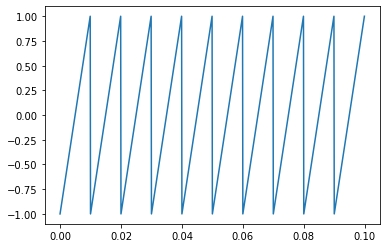
\includegraphics[width=\textwidth]{ex6_first.png}
        \caption{Пилообразный сигнал}
        \label{fig:ex6_first}
    \end{figure}
    
\begin{lstlisting}[language=Python,caption=Его спектр]
spectrum = wave.make_spectrum()
spectrum.plot()
\end{lstlisting}

    \begin{figure}[H]
        \centering
        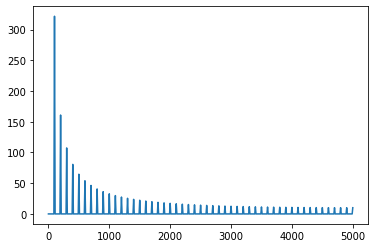
\includegraphics[width=\textwidth]{ex6_first_spectrum.png}
        \caption{Спектр}
        \label{fig:ex6_first_spectrum}
    \end{figure}
    
    Применим \texttt{modify()}.
    
\begin{lstlisting}[language=Python,caption=Снова применяем \texttt{modify()}]
modify(spectrum)
spectrum.plot()
\end{lstlisting}

    \begin{figure}[H]
        \centering
        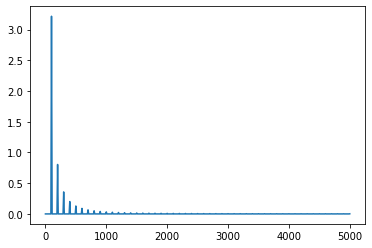
\includegraphics[width=\textwidth]{ex6_second_spectrum.png}
        \caption{Модифицированный спектр}
        \label{fig:ex6_second_spectrum}
    \end{figure}
    
    Посмотрим, что там вышло.
    
\begin{lstlisting}[language=Python,caption=Смотрим]
wave2 = spectrum.make_wave()
wave2.plot()
\end{lstlisting}

    \begin{figure}[H]
        \centering
        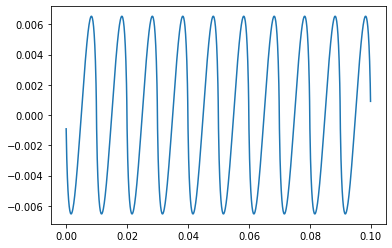
\includegraphics[width=\textwidth]{ex6_second.png}
        \caption{Видим}
        \label{fig:ex6_second}
    \end{figure}
    
    Похоже на синусоиду, но это точно не она. Иначе бы спектр содержал лишь одну компоненту. Признаюсь, я так и не догадался сам, поэтому посмотрел в решение - там написано, что это \texttt{ParabolicSignal}.
    
\begin{lstlisting}[language=Python,caption=Что же это за сигнал такой...]
from thinkdsp import ParabolicSignal

signal4 = ParabolicSignal(100)
wave4 = signal4.make_wave(duration=signal4.period*4, framerate=10_000)
wave4.plot()
\end{lstlisting}

    \begin{figure}[H]
        \centering
        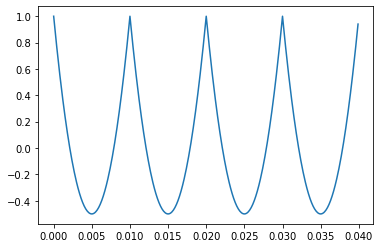
\includegraphics[width=\textwidth]{ex6_third.png}
        \caption{Вот это я понимаю сигнал}
        \label{fig:ex6_third}
    \end{figure}

\end{document}
